\title{\textbf{\Huge Book-taste clustering in goodreads communities}}

\author{{\Large Akanksha Tiwari (A0123476E)} \\
    {\Large Antoine Francois Pascal Creux (A0123427M)}\\
    {\Large Ashish Dandekar (A0123873A)} \\\\
    National University of Singapore,\\
    Singapore
}
\date{\today}

\documentclass[11pt]{article}
\usepackage[margin=1in]{geometry}
\usepackage[english]{babel}
% \usepackage{listingstyle}
\usepackage{graphicx}
\usepackage{caption}
\usepackage{subcaption}
% \usepackage{coz}
% \usepackage[sorting=none]{biblatex}
\usepackage{url}
\usepackage{array}
\usepackage{multirow}
\usepackage{soul}
\usepackage{amssymb}
\usepackage{hyperref}
% \usepackage[autolanguage]{numprint}

\begin{document}
\maketitle

\section{Detailed Problem Description}
Goodreads is a website launched in early 2007, which lets ``people find and share the books they like and improve the process of reading and learning throughout the world.'' It is the world's largest site for readers and book recommendations with a user base of about 30 million members along with 34 million reviews from 900 million books as recorded in 2015 \footnote{\url{http://www.goodreads.com/about/us}}.\\\\
Goodreads provides a multitude of features to its users. It goes beyond the traditional rating and reviewing of books by allowing users to make friends and join and form reading groups based on their literary tastes.
Users can not only see what their friends have read, but they can also meet new people with similar reading interests. They can make recommendations to friends, follow authors, track the books they are currently reading, have read and want to read. In addition, goodreads provides personalized recommendations to book readers by analyzing the user data.\\\\
Our project aims  to detect and study goodreads communities based on the book ratings given by users. Through this analysis we seek to understand whether the communities detected based on similar book tastes are alike to the friends communities formed by users themselves on goodreads and the extent to which these user communities on goodreads exhibit homophily.
\subsection{Assumptions}
% zero rating

The users who have not provided any ratings for the books that they have read are considered as invalid users and we have eliminated them from our data set. This is because just having read the book does not indicate that the user has liked the book. We also need the rating he has given to the book to know whether he/she likes(high rating) or dislikes (low rating) the book he has read.\\\\
The users with private profiles whose data we could not scrape because their reading information is just visible to their friends are also considered as invalid users. So, we have not included them in our data set.\\\\
We are assuming that the data we get from scraping is unbiased. That is, we assume that the group ({\it Goodreads Authors/Users}) whose members, members' friends and their books read that we have scraped is representative of readers from various genres. Indeed, this group is very large and popular and is used to share book experiences across different genres.

\subsection{Objectives}

\begin{itemize}
\item[\checkmark] Gather relevant data (as mentioned in Section \ref{sec:data_acquisition}) from goodreads
\item[\checkmark] Survey various algorithms for community detection on the graphs generated from the data
\item[\checkmark] Analyze and interpret the results of applying these algorithms on the data 
\item[\checkmark] Analyze the extent to which the user groups on goodreads exhibit homophily
\item Study the effect of recommendations and users' friend on his/her choice of books (If time permits)
\end{itemize}

\subsection{Contribution}
As of the literature survey done up to now, there has not been a study on the detection of communities of readers with similar reading interests on goodreads dataset.
This work will aim to identify such communities using algorithms for community detection such as Louvain algorithm and compare the communities detected with the already formed groups on goodreads and analyze how different or similar they are.
This would give us insights into whether the friendship and groups formed on goodreads are based on reading interests or there are other factors that come into play. It can be especially useful to authors in identifying the right target audience for their work. \\\\

\section{Related Work}
Community detection is a widely discussed topic in the social networking literature\footnote{Social networks are generally sparse networks. When the networks are dense, the community detection does not seem to be a wise option. The dense networks possess large number of inter-community edges which yield poor partitioning. For dense networks, discrete data analysis techniques are used.}\cite{survey}. {\it igraph}\cite{igraph} provides implementation of a number of community detection algorithms\cite{r-bloggers} - Girvan-Newman, Louvain, Label propagation and Fast-greedy.\\\\
Initially, we decided to use the Girvan-Newman algorithm as it is one of the most popular community detection algorithms\cite{girvan}. This algorithm uses the ``edge betweenness'' of an edge as the number of shortest paths between pairs of nodes that run along it. Edges with high betweenness are very likely to be the connection between communities.
Thus, removing the edges in the decreasing order of betweenness should reveal the associated dendrogram, and thus the communities. However, this computation takes $O(ne)$ running time, and thus is too long for our graph.\\\\
The Louvain\cite{louvain} method for community detection which has come up in the last few years, is a graph partitioning technique that provides an accurate and computationally efficient approach to detect communities through greedy optimization in networks consisting of millions of nodes. It optimizes the modularity of a partition of a network. Wikipedia defines modularity as ``The fraction of the edges that fall within the given groups minus the expected such fraction if edges were distributed at random''. This is an agglomerative community detection approach where first, every node is assigned to its own community. Subsequently, the change in modularity is calculated for moving that node from its own community into the community of each of its neighbors and the node is then put in the community that resulted in the maximum increase in modularity. Next, the nodes that are part of the same community are aggregated  and then another network is constructed whose nodes are the communities. These steps are repeated till the modularity is maximized.\\\\
Like Louvain, fast-greedy\cite{clauset} is also a hierarchical agglomerative community detection algorithm. However, louvain is more efficient for graphs with large number of nodes as it optimizes the modularity more efficiently.   
Another community detection algorithm is the label propagation algorithm\cite{propagation} which relies neither on divisive nor agglomerative clustering. It just uses the network structure and does not use optimization of any pre-defined objective function. In this algorithm, initially, each node is given a unique label. However, at every iteration each node picks a label that a maximum number of its neighbors has (with ties broken uniformly randomly). In this way, densely connected groups of nodes  create an agreement on their labels. At the end, nodes which have same labels are clustered together in communities. Since this is a randomized algorithm a number of community structures are possible starting from the same initial condition.\\\\
Community detection algorithms can also be classified as: member based algorithms and group based algorithms. Member based algorithms use the properties of the nodes to find the communities in the network whereas group based algorithms use the connectivity in the network to detect the communities. In the current study, we have taken a hybrid approach. We use the properties of the nodes to generate the network and later use group based algorithms to find the communities.
\section{Data Acquisition}
\label{sec:data_acquisition}
Goodreads provides well documented and publicly accessible APIs to query various features supported by the website. All we need is a developer key, which one gets after signing up on goodreads, and an OAuth access to use numerous APIs. The data of the users on a website, being the concern of privacy, is not readily available by means of goodreads APIs. Aside from this a goodreads user has liberty to keep his/her profile private making it accessible only to his friends on goodreads. Given the large user-base of goodreads, we hope to get sizable dataset to run our analysis.\\\\
Although the data scraping is laborious and time consuming, its is vital in our study. For a fair study, the data must be unbiased. The method which we use to gather the data may add some bias to it. So selection of scraping method is critical to data acquisition. There are two ways one can collect the data:
\begin{description}
\item[Retrieve User IDs from a group]
Goodreads hosts various reading groups catered to various genres and reading interests. User can become member of such groups or can initiate a group. In a group reading activities are supported wherein members can schedule the book readings so that they can share their opinions and conduct a healthy conversation. {\it Goodreads Authors/Readers} is one of the major groups on goodreads.  According to goodreads, this group is dedicated to connecting readers with goodreads authors. It is divided by genres, and includes folders for writing resources, book websites, videos/trailers, and blogs. A {\it toy dataset} scraped from the group shows the absence of bias in the data.\\
Goodreads provides an API to get the list of users given the ID of the group. One can get the ID of the group from the URL of the corresponding group on goodreads.
\item[Retrieve User IDs from reviews of books]
The list of various books genres is available at \footnote{\url{http://www.goodreads.com/genres}}. One can select top rated books from the highly reviewed genres. So this collection of ``best-selling'' books forms a base set for the books. So we can get the list of users who have read these books. But goodreads fails to support an API which retrieves reviews for a particular book given its ID. Despite this, a meticulous analysis of \textit{Javascript} calls, the webpage makes to show the reviews of a book to the user, reveals a bacdoor API \textit{book/reviews/}. We can retrieve user related information User ID and the rating by parsing the response to the \textit{Javascript} callback using regular expression.

\end{description}
The list of User IDs thus scraped serve as a base user set. We later collect {\it 1-neighbourhood} of this set of users, namely friends of them and the books read by these friends, to get a substantial dataset.\\
We are using the first strategy to scrape the data off the goodreads. Plus the data related to the friends assures the sizable amount for the analysis.

\subsection{Statistics}

An overview of the goodreads data we have scraped is vital as it helps us understand and grasp insight of the data we are munging.
As described in this section earlier, we have extracted our data in two steps:
\begin{itemize}
\item Members of the Goodreads Authors/Users
\item Friends of the Goodreads Authors/Users members
\end{itemize}

\begin{table}[ht]
\begin{center}
\begin{tabular}{lcccc}
\hline
                           &  Goodreads Authors/Users    &   Friends                &   All        \\ \hline
\#Ratings                  &  567461                     &   13832047               &   14399503  \\ \hline
\#Users                    &  17583                      &   95503                  &   113086     \\ \hline
\#Public Profiles          &  7816                       &   78723                  &   86538     \\ \hline
\#Private Profiles         &  2564                       &   5314                   &   7878      \\ \hline
\#Profiles w/o any reviews &  7203                       &   11559                  &   18762      \\ \hline
\#Books rated              &  171653                     &   11559                  &   1714613      \\ \hline
\end{tabular}
\end{center}
\caption{Goodreads Authors/Users Statistics} \label{table:crawl_stat}
\end{table}
% Problem with private profiles. Need data from 100 to 350 for 1st degree connection
% But akanksha has already uploaded the 100 to 350 data
As we can see, by getting only the first degree connection of approximately twenty thousand members of {\it Goodreads Authors/Users} group, we have close to 15 million reviews, 1714613 books and 86000 users to analyze.

%\begin{figure}
%        \centering
%        \begin{subfigure}[b]{0.5\textwidth}
%                %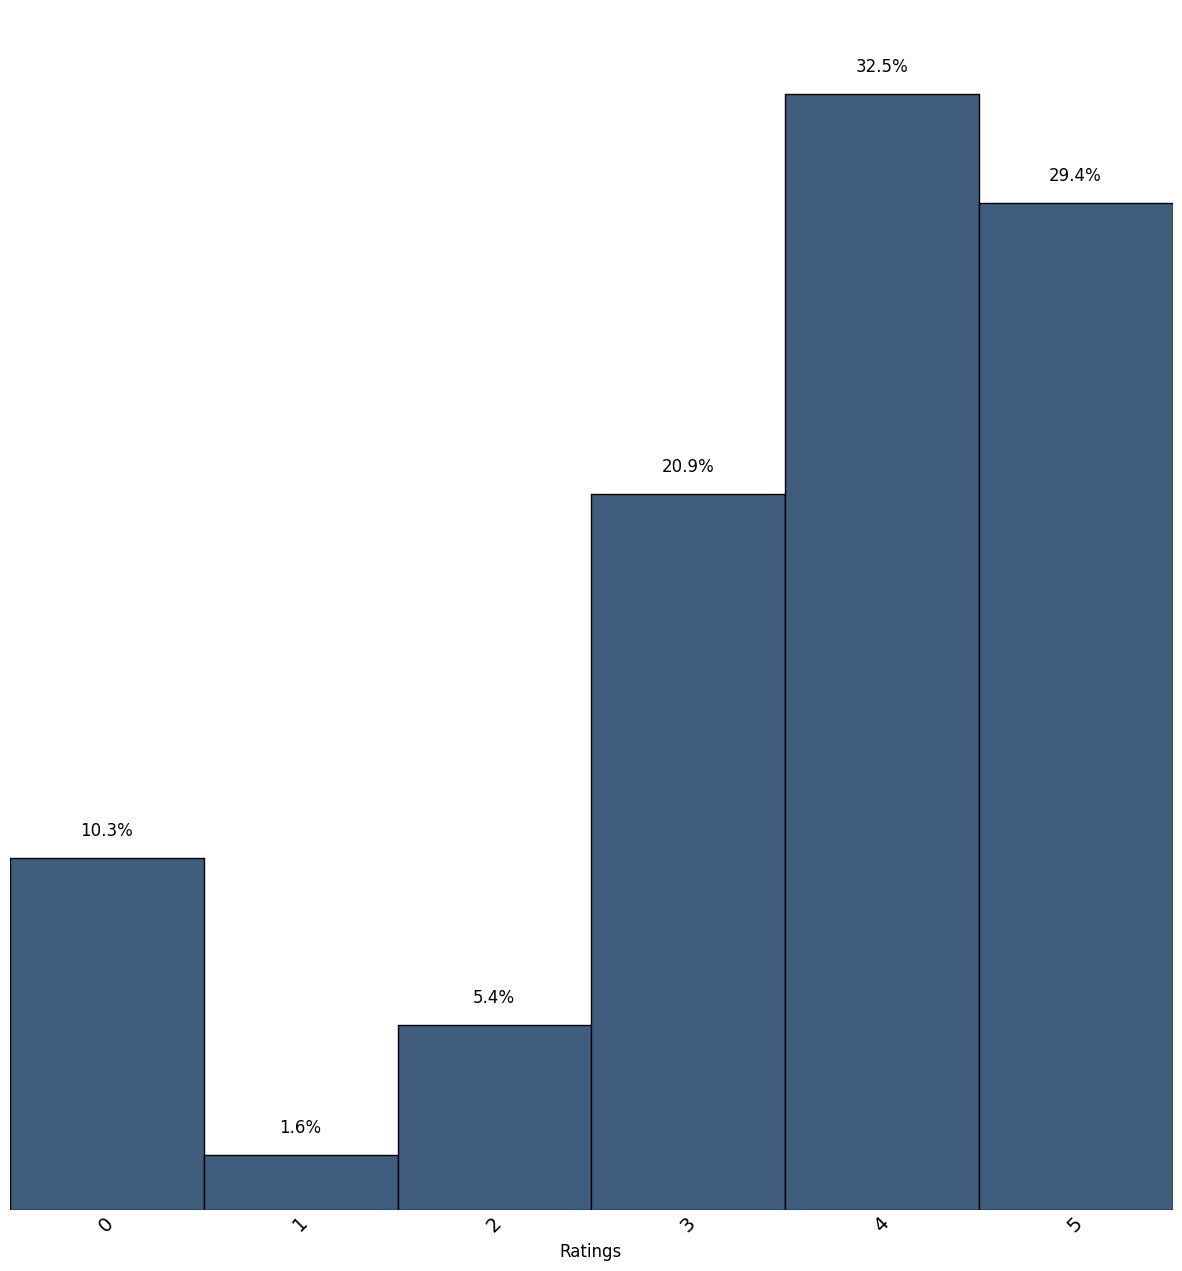
\includegraphics[width=\textwidth]{all_ratings}
%                \label{fig:all_reviews}
%        \end{subfigure}%
%        \caption{Distribution of reviews}
%\end{figure}
Let's observe a few things in the base dataset. Users have read an average of $166$ books, whereas a book has been read by an average of $8$ people. Please refer to Figure~\ref{fig:readers_book_read} to see the detailed user statistics. There is a large portion of the readers which has read less than 50 books. Figure~\ref{fig:books_books_read} shows the stats for the books. $54.2\%$ books in the dataset are read/reviewed by a single user. Only $10$\% of the books have been read by more than $10$ readers. This stark contrast separates the books which are popular from the ones which are not much popular. Users have given an average rating of $3.52$ to the books while books have an average of $3.23$.

% print c.user_average_book()
% print c.book_average_user()
% print c.user_average_rating()
% print c.book_average_rating()

% 166.39514433
% 8.38730595677
% 3.524460734
% 3.22690806765

\begin{figure}[ht]
        \centering
        \begin{subfigure}[b]{0.5\textwidth}
                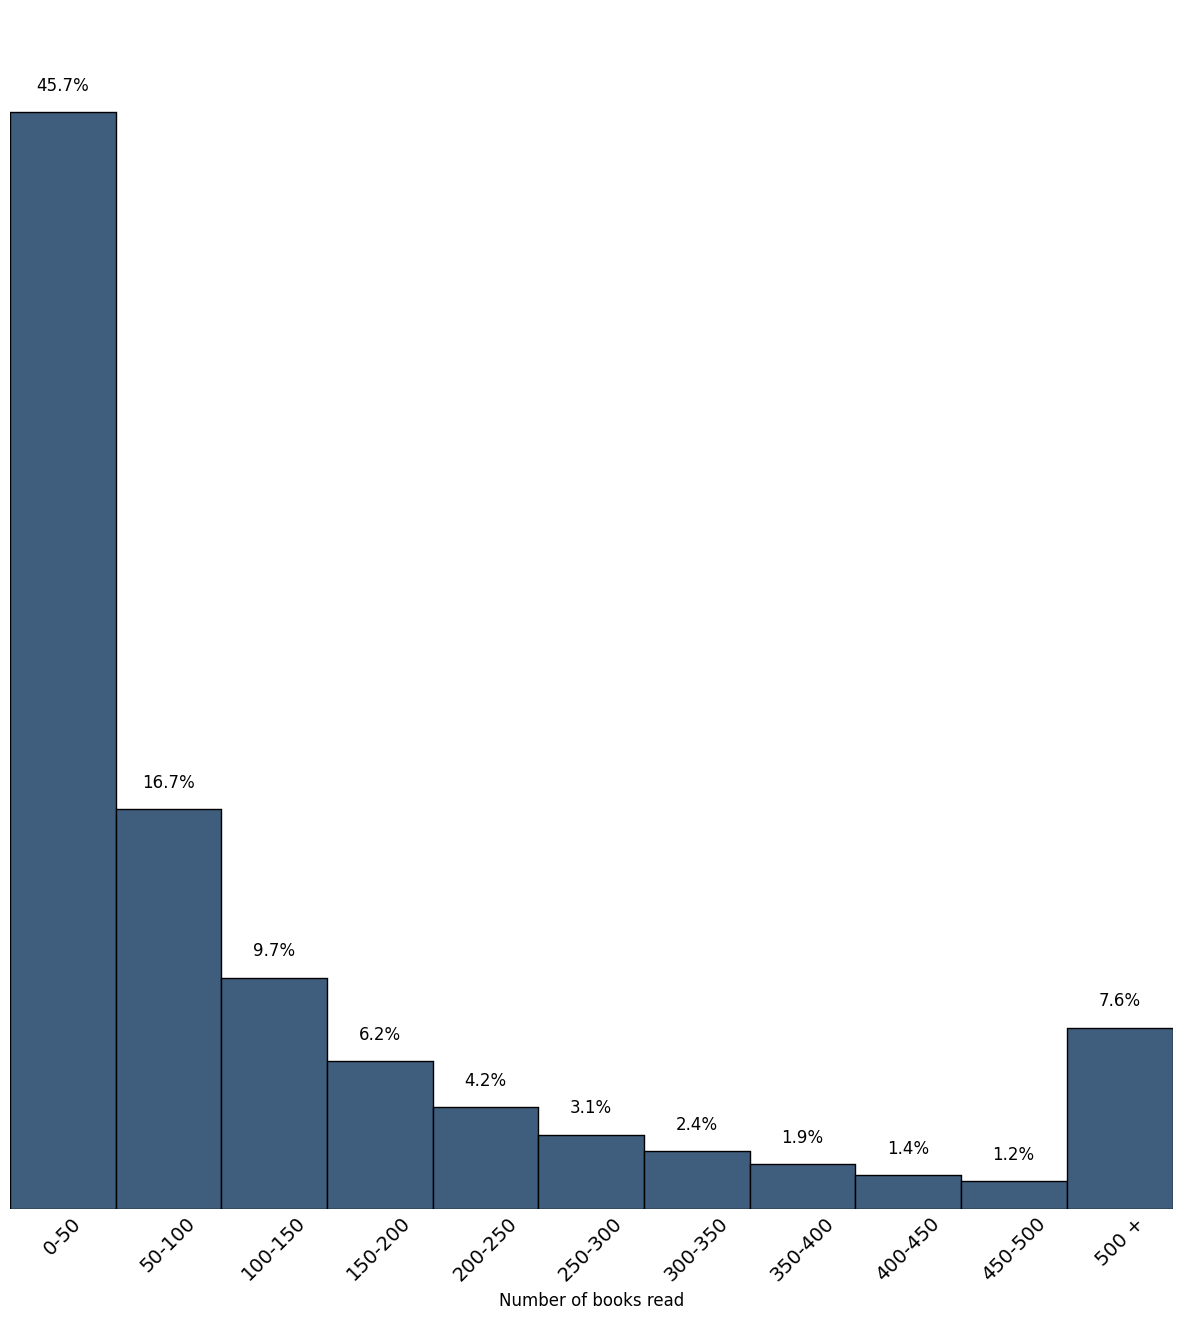
\includegraphics[width=\textwidth]{users}
                \caption{Distribution of readers}
                \label{fig:readers_book_read}
        \end{subfigure}%
        ~ %add desired spacing between images, e. g. ~, \quad, \qquad, \hfill etc.
          %(or a blank line to force the subfigure onto a new line)
        \begin{subfigure}[b]{0.5\textwidth}
                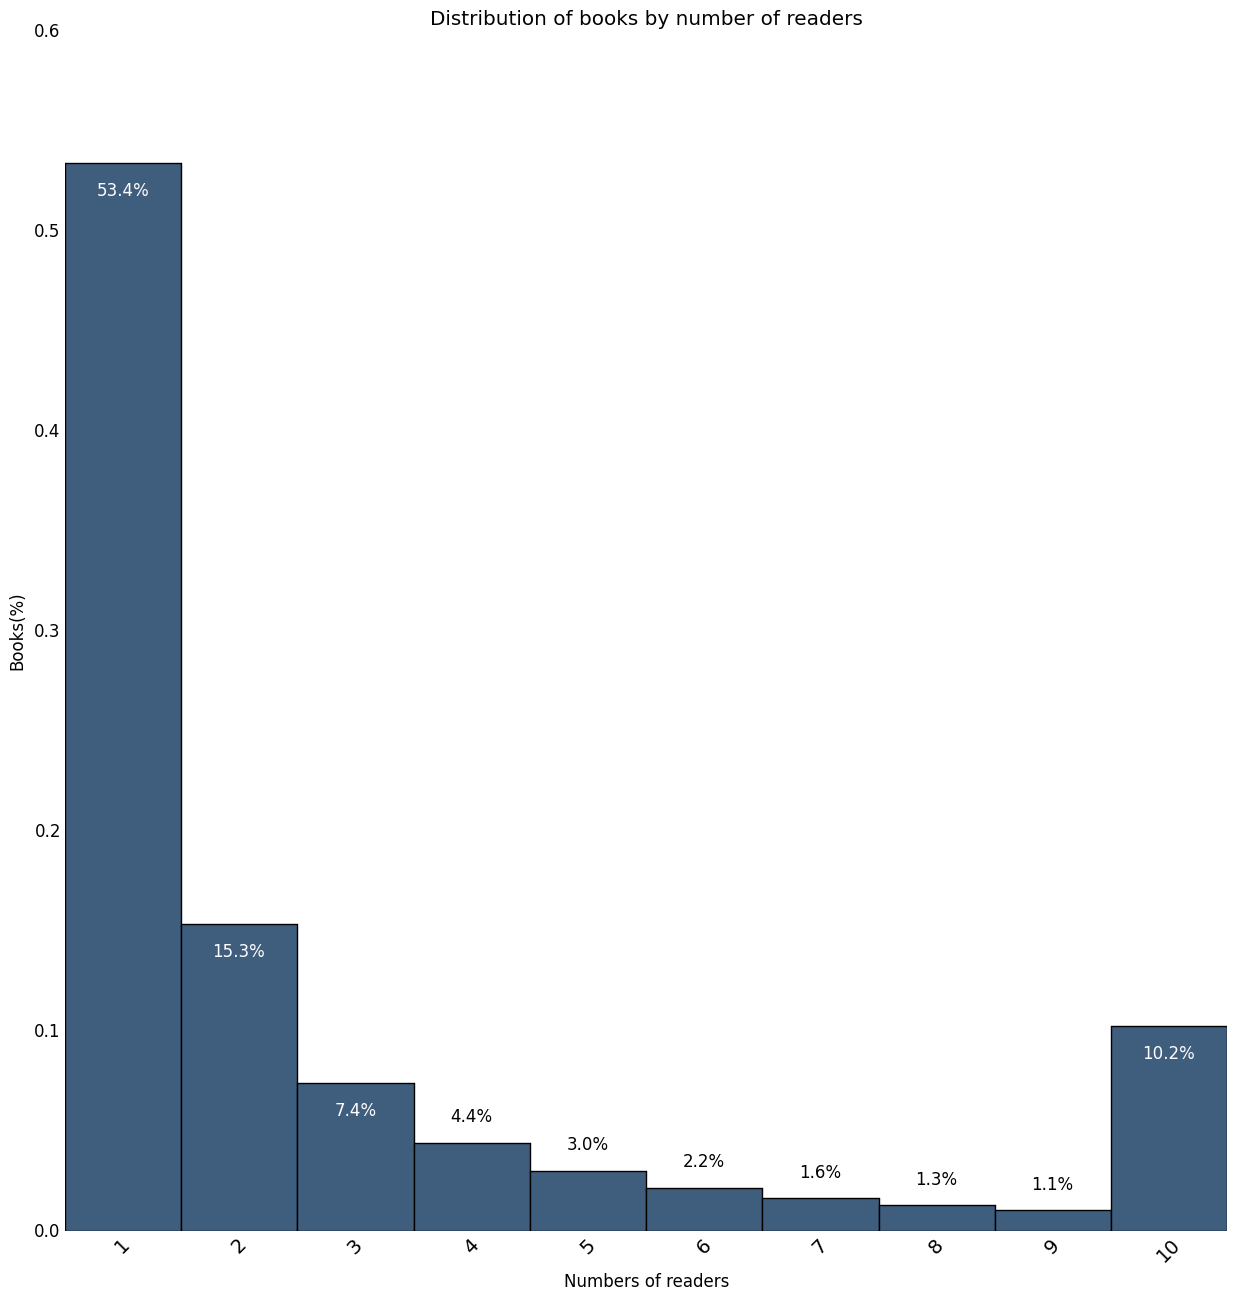
\includegraphics[width=\textwidth]{books}
                \caption{Distribution of books}
                \label{fig:books_books_read}
        \end{subfigure}
        \caption{Distribution of books and readers}
\end{figure}

% Books read: 1714613

% !!!!!!always fix bucket size of the column depending on the data!!!!

% User to book
% ------------

% column chart 
% average How many books a user has read - - I want total average



\begin{figure}
        \centering
        \begin{subfigure}[b]{0.5\textwidth}
                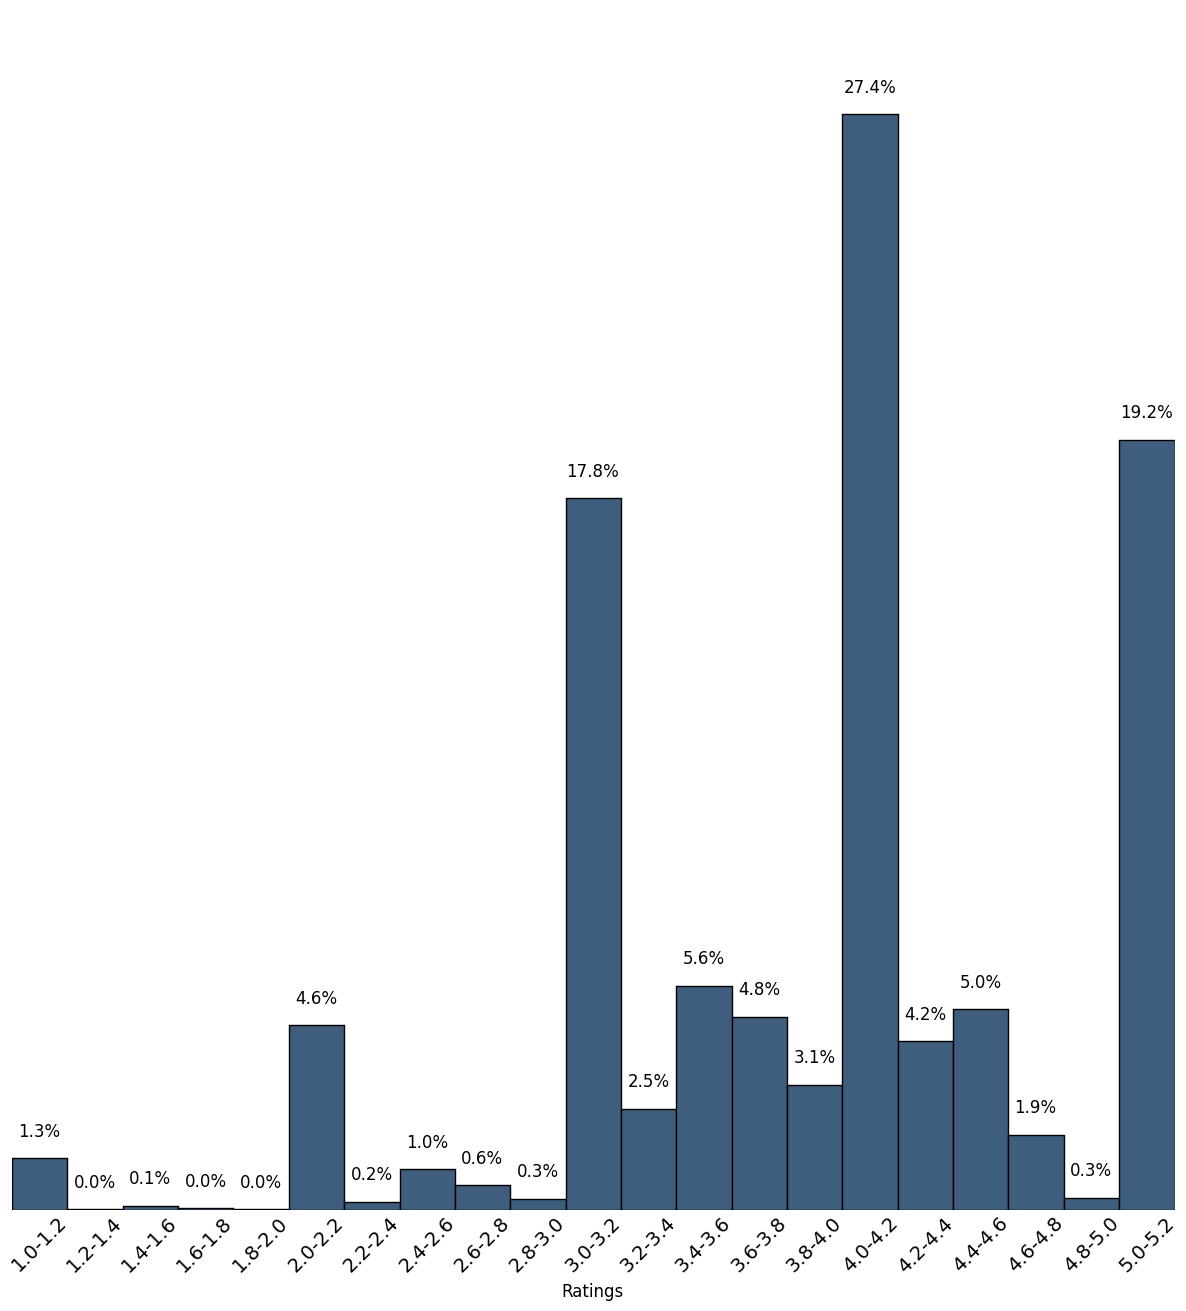
\includegraphics[width=\textwidth]{books_ratings}
                \caption{Distribution of books}
        \end{subfigure}%
        ~ %add desired spacing between images, e. g. ~, \quad, \qquad, \hfill etc.
          %(or a blank line to force the subfigure onto a new line)
        \begin{subfigure}[b]{0.5\textwidth}
                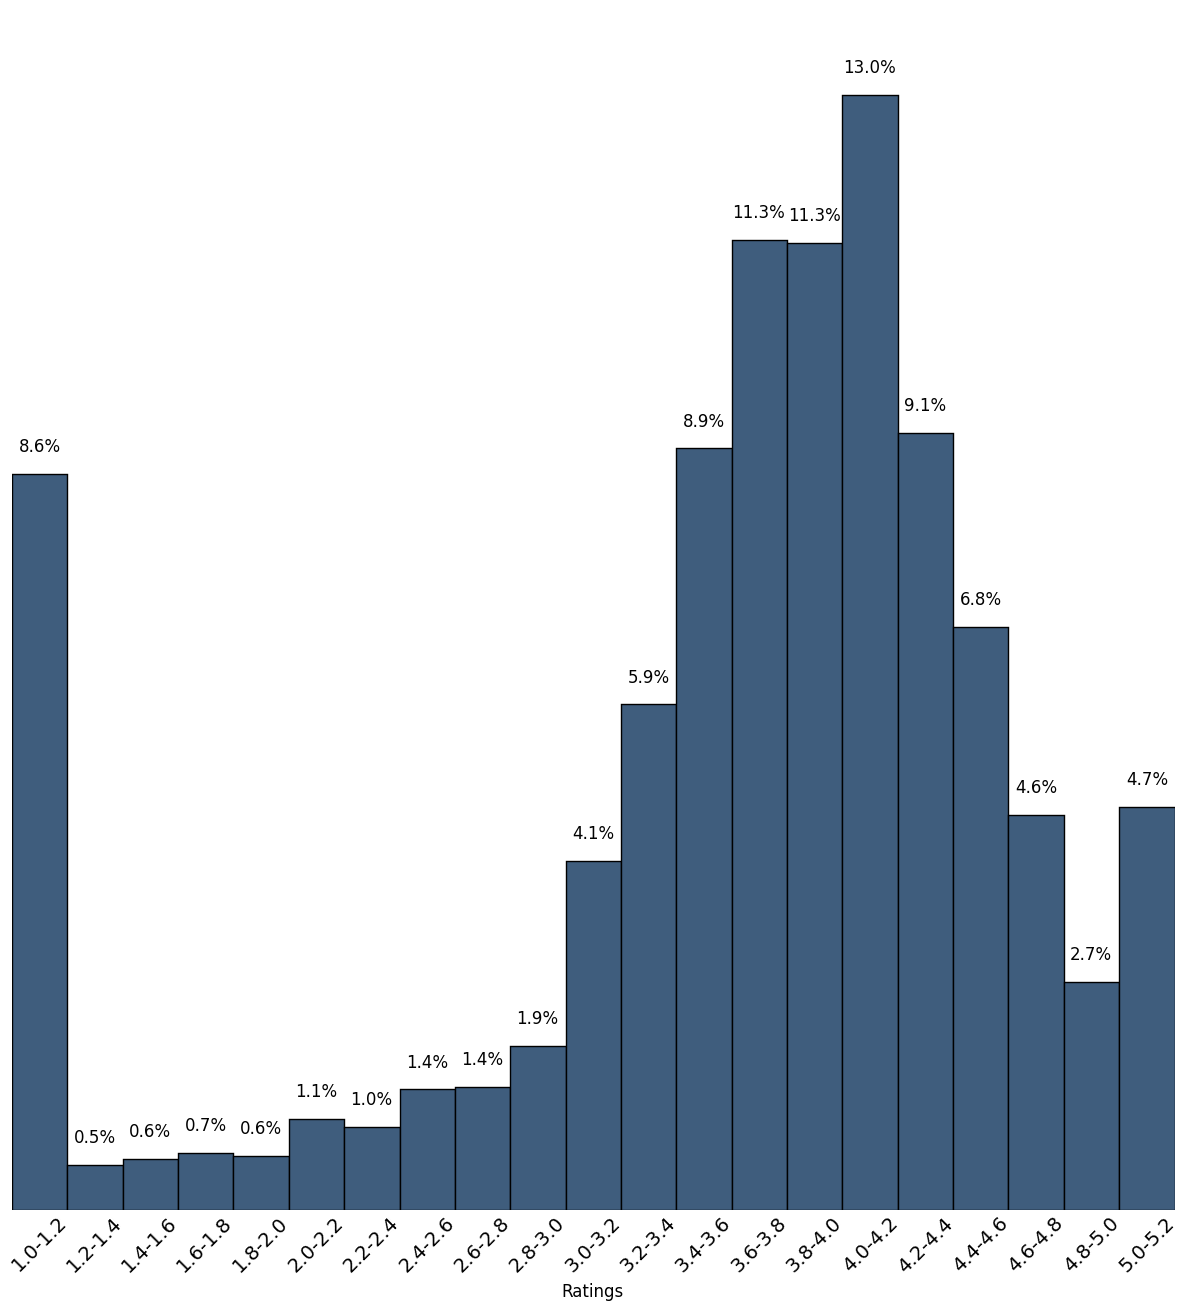
\includegraphics[width=\textwidth]{user_ratings}
                \caption{Distribution of readers}
        \end{subfigure}

%         \begin{subfigure}[b]{0.5\textwidth}
%                 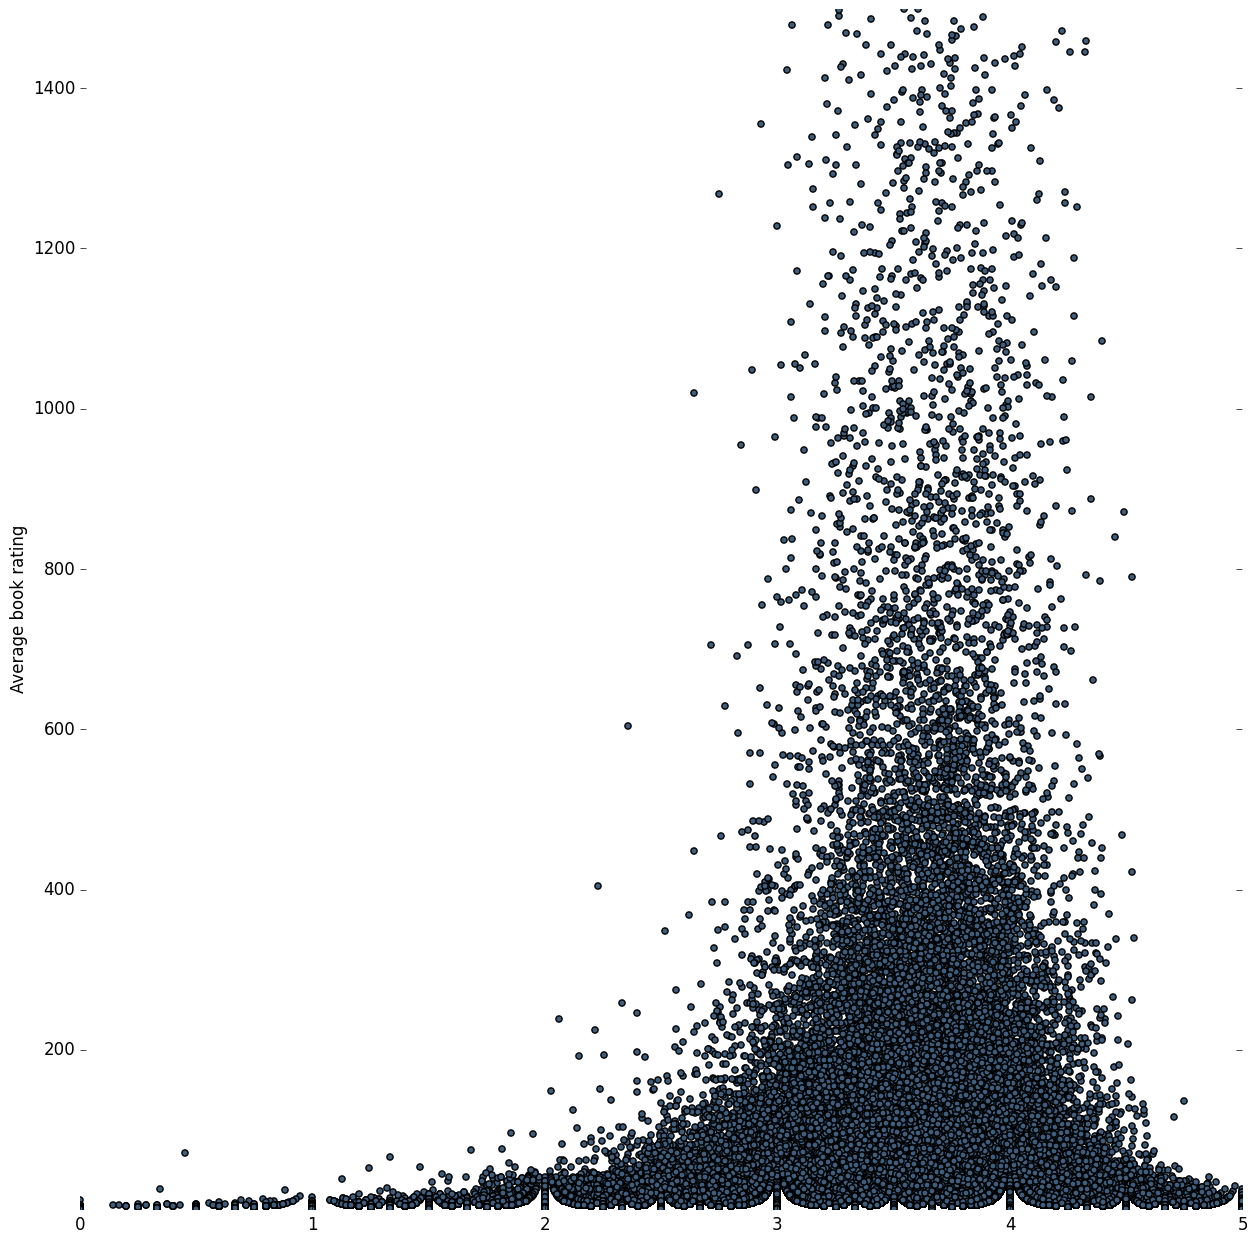
\includegraphics[width=\textwidth]{book_scatter_1500}
%                 \caption{Books per rating}
%         \end{subfigure}%
%         ~ %add desired spacing between images, e. g. ~, \quad, \qquad, \hfill etc.
%       %(or a blank line to force the subfigure onto a new line)
%         \begin{subfigure}[b]{0.5\textwidth}
%                 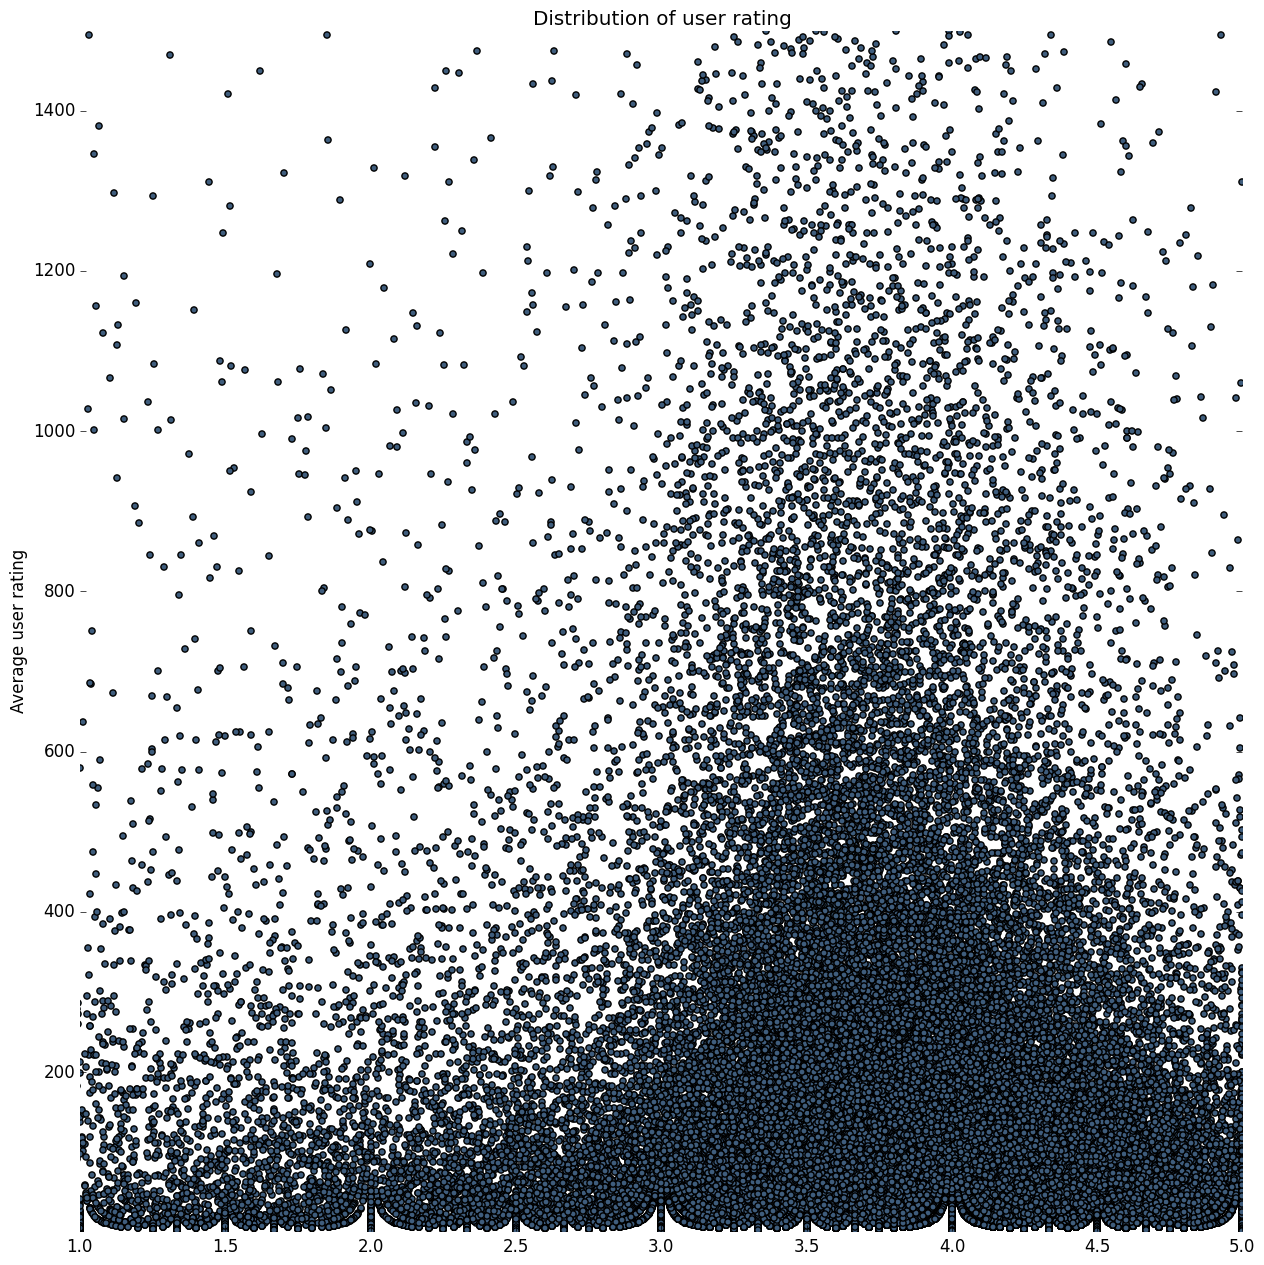
\includegraphics[width=\textwidth]{user_scatter_1500}
%                 \caption{Readers per rating}
%         \end{subfigure}
        \caption{Distribution of ratings for readers and books}
        \label{fig:scatters}
\end{figure}

About the distribution of ratings, both books and readers have a similar distribution as seen in Figure~\ref{fig:scatters}.


\section{Description of the method}
\label{sec:method}
% Right about score functions - sab kuch
\subsection{Score Function}
As stated earlier, the objective of the current study is to explore the homophily in the goodreads network. Homophily, the concept in the Social Network Analysis, tries to reason the existence of ties among different vertices in the network. Homophily says that the ties exist between the vertices which share similar properties. The kind of properties, a vertex has, depends on the type of social network under the study. For instance, in a citation network the research domain of the authors serve as the property a vertex possesses whereas in an online dating network the hobbies, mutual interests of the users are the driving force for initiating ties among the users. Goodreads network not only has reading groups of users but also has the provision to become a friend of user. In this study, we want to reason the ties which goodreads have as a part of friendship graph.\\\\
One can think about many reasons which leads a user to connect another user on goodreads. We need to quantify this notion so as to make observations. We use different score functions while generating a user-user graph from the scraped data. Each score function quantifies a kind of homophily which we want to study. We have considered following score functions.
\begin{description}
	\item[Common Books] Given two users, we establish an edge between the users if and only if both of the users have read {\it threshold} number of books in common. We can tune the threshold to get the extent of homophily.
    \item[Common Books Normalized] Given two users, the homophily is defined by the number of books both users have read in common, normalized by the number of books both users have read in total.
    \item[Rating Based]It builds on the earlier score by incorporating the rating given by the users to the books they have read. We add an edge between the users if the users have given {\it similar}\footnote{For instance, ratings differ by one} ratings to at least {\it threshold} fraction of the books they have read.
    \item[High Rating Based] This score behaves the same as \textit{Rating Based} except we give a higher weight to high scores. If both of the users have given high rating the tie strength increase.
\end{description}
First score function shows how similar books user have read whereas the second score function is more subtle looking at whether the users have liked the books they have read. We construct user-user graphs using these score functions and scraped data.

\subsection{Sampling}
We want to find the communities in the user-user graph formed in this way. Nonetheless, the number of users is prohibitive to obtain the communities in the network in considerable amount of time. A few techniques can be employed to reduce the number of users:
\begin{description}
	\item[Reviews Sampling] Instead of considering all of the sampled data, we consider fraction of edges between user and book. Random sampling fails to capture important users since this technique may not consider all the books which a user has read
    \item[Users Sampling] In this technique, we directly sample desired number of users from a set of users. Then we use all the books read by the sampled set of users to create user-user matrix.
    \item[Active Users] It can be clearly observed that, there is a large fraction of users who have read very few books. It may be advantageous to focus the study on voracious readers. These are the reader who have read many books and reviewed them. We can choose the users who have read at lest $k$ books. One can tune $k$, to get desired number of users.
     \item[Edges Filtering] Even after sampling the readers, a $10000$ readers sample can generate 25 million edges if the user-user graph density is still $50\%$. Given that each edge has a score, we can filter them and take the $n$ highest edges.
\end{description}
We have implemented {\it user sampling} and {\it active users} method to restrict the number of users.




% \subsection{Sampling}
% We want to find the communities in the user-user graph formed in this way. Nonetheless, the number of users is prohibitive to obtain the communities in the network in considerable amount of time. A few techniques can be employed to reduce the number of users:
% \begin{description}
% 	\item[Reviews Sampling] Instead of considering all reviews, we can consider only a fraction of them. However, random sampling fails to capture important users since this technique may not consider all the books which a user has read. We did \textbf{not} use it.
%     \item[Users Sampling] In this technique, we directly sample desired number of users from a set of users. Then we use all the books read by the sampled set of users to create user-user matrix. This sampling method is fair.
%     \item[Active Users] It can be clearly observed that, there is a large fraction of users who have read very few books. It may be advantageous to focus the study on voracious readers. These are the readers who have read many books and reviewed them. We can choose the users who have read at least $k$ books. One can tune $k$, to get desired number of users.
%     \item[Edges Filtering] Even after sampling the readers, a 10000 readers sample can generate 25 million edges if the user-user graph density is still 50\%. Given that each edge has a score, we can filter them and take the $n$ highest edges.

% \end{description}
% We have implemented {\it users sampling}, {\it active users} and {\it edges filtering}.










\subsection{Community Detection}
Once the communities are found we proceed to calculate homophily in the network. To calculate the homophily, we use the friendship information related to users. Let $S$ denote the set of users in a graph and $f(u)$ denotes set of friends of user $u$($\in S$) in $D$. Let $\mathcal{C}$ be the set of communities returned by community detection algorithm. Homophily of cluster $C_i$ is calculated as:
\[
\mathcal{H}_{C_i} = \sum_{v \in C_i} \frac{|C_i \cap f(v)|}{|f(v)|}
\]
We use the homophily of the cluster to find global homophily for the graph. It is weighted sum of cluster homophily. It is given by:
\[
\mathcal{H}_{S} = \sum_{C_i \in \mathcal{C}} w_{C_i} \mathcal{H}_{C_i} ~~~~~~~~~\textrm{where,}~~~w_{C_i} = \frac{|C_i|}{|S|}
\]
Since the homophily calculation relies heavily on the community detection algorithm, use of a single community detection algorithm may make the analysis biased. So as not to make the analysis partisan we use two different algorithms for analyzing user-user graph.\\\\
In this way, {\it Score Function}, {\it Sampling} and {\it Community Detection} are the dimensions along which we analyze the homophily in goodreads community.

\section{Challenges}
We encountered many challenges at different stages of the project. Here we enlist them one by one.

\subsection{Data processing}
Each information needs a request to goodreads to fetch the data. To gather data related to a user, namely friends and books, a lot of queries have to be fired to goodreads. For close to $86000$ users, we made more than 1 million requests. We used multiprocessing to expedite this process.

\subsection{Matrix projection}
We need to generate user-user matrix from a bipartite network comprising of approximately $86000$ users, $1.7$ million books and $14$ million edge. Although the bipartite network is sparse, the resultant one mode projection is highly dense. When we got memory issues with {\it networkX}\cite{networkx} we used {\it scipy}\cite{scipy} as a resort. But even with scipy, the projected matrix being very dense, memory issues persisted\footnote{ We hit a memory overflow on a machine with 64GB of main memory.}. Plus the community detection algorithms have very poor running time for large graphs. To skip both of these hurdles, we used sampling techniques as described in Section \ref{sec:method}

\subsection{User-User Graph}
Use of matrix multiplication is a classical way to compute one mode projection. But the objective of the study is directed more towards semantics of the ties, we compute each edges between two users by hand making use of score functions defined in Section \ref{sec:method}. As we need to compute the edge weight between every pair of two readers, to build a graph with $n$ users, we must iterate over $n \choose 2$ edges. For 10000 users, we have to compute 50 million edges. Again we use multiprocessing, to expedite this user-user graph generation.

\subsection{Community Detection Algorithms}
Once we have created user-user graph, finding communities in the graph is part of the analysis. Finding communities in the graph is a computationally expensive process. First of all, the underlying graph must fit inside main memory. With large and dense networks, we had memory issues a few times in {\it NetworkX}. So, we switched to {\it igraph} library\cite{igraph}. It is a very efficient library implement in C and provides interface in many languages such as Python, R. Not just the library is highly efficient but many community detection algorithms have, already, been implemented in {\it igraph}.


\section{Evaluation}

As described in Section \ref{sec:method}, we have done analysis based on three metrics: user sampling technique, score function and community detection algorithm. The analysis results are tabulated in Table \ref{table:analysis_stat}. The analysis has been run on a sample of $5000$ users. In {\it random} case, $5000$ users have been randomly sampled. In {\it active} case, the {\it user significance} was tuned to $600$(this means that we consider only those users who have read more than $600$ books) to obtain a sample $5000$ users. We have also done analysis by choosing various thresholds for each score function technique. But due to lack of space we are listing the results for threshold of 0.7 in case of {\it rating}(meaning that at least $70\%$ of the books have been given similar rating) and threshold 30 in case of {\it score}(meaning that users have read at least 30 common books). We have conducted the analysis for other scoring functions as well. In the Table \ref{table:analysis_stat}, we have listed two of them.


\begin{table}[h]
\begin{tabular}{|l|l|l|l|l|l|l|}
\hline
\multicolumn{1}{|c|}{\textbf{Sampling}} & \multicolumn{1}{c|}{\textbf{Score}} & \multicolumn{1}{c|}{\textbf{Edges}} & \multicolumn{1}{c|}{\textbf{Friends}} & \multicolumn{1}{c|}{\textbf{Algorithm}} & \multicolumn{1}{c|}{\textbf{Clusters}} & \multicolumn{1}{c|}{\textbf{Homophily}} \\ \hline
\multirow{6}{*}{Random} & \multicolumn{1}{c|}{\multirow{3}{*}{Rating}} & 2,601,610 & 11,784 & Louvain & 4 & 0.1876 \\ \cline{3-7} 
 & \multicolumn{1}{c|}{} & 2,601,610 & 11,784 & FastGreedy & 7 & 0.2798 \\ \cline{3-7} 
 & \multicolumn{1}{c|}{} & 2,601,610 & 11,784 & Label Propagation & 1 & 0.4576 \\ \cline{2-7} 
 & \multirow{3}{*}{Common} & 106,815 & 4,758 & Louvain & 8 & 0.1770 \\ \cline{3-7} 
 &  & 106,815 & 4,758 & FastGreedy & 11 & 0.0242 \\ \cline{3-7} 
 &  & 106,815 & 4,758 & Label Propagation & 5 & 0.0896 \\ \hline
\multirow{6}{*}{Active} & \multirow{3}{*}{Rating} & 4,244,161 & 122,714 & Louvain & 3 & 0.5107 \\ \cline{3-7} 
 &  & 4,244,161 & 122,714 & FastGreedy & 3 & 0.5697 \\ \cline{3-7} 
 &  & 4,244,161 & 122,714 & Label Propagation & 1 & 0.9017 \\ \cline{2-7} 
 & \multirow{3}{*}{Common} & 5,461,898 & 122,414 & Louvain & 5 & 0.6589 \\ \cline{3-7} 
 &  & 5,461,898 & 122,414 & FastGreedy & 6 & 0.1126 \\ \cline{3-7} 
 &  & 5,461,898 & 122,414 & Label Propagation & 2 & 0.4496 \\ \hline
\end{tabular}
\caption{Goodreads Authors/Users Statistics}
\label{table:analysis_stat}
\end{table}

%edges/active_edges_common_600_20.csv    friends:  235296
%edges/active__edges_common_600_30.csv    friends:  235296
%edges/active_edges_rating_600_0_5.csv    friends:  235881
%edges/active_edges_rating_600_0_7.csv    friends:  235881
%edges/random_edges_common_5000_20.csv    friends:  11733
%edges/random_edges_common_5000_30.csv    friends:  8910


From the numbers we have got following observations can be made:
\begin{itemize}
	\item It can be clearly seen that we have got the higher homophily scores for {\it active} user sample. These are the users who have read more than $600$ books. So, it is likely that they might have read large number of common books. Since the score functions rely on the common books they have read they the high scores might have resulted from this bias.
    \item We have created the user-user graph using score functions and the thresholds. Despite this, the overlap between the goodreads friendship network and the user-user graph is very small. This implies that the friendship ties do not adhere to either of the score functions.
    \item Even with different algorithms, the global homophily scores are not enlightening enough to conclude the relationship between the score function and the homophily in the goodreads network.
\end{itemize}
From these observations, we can say that the book-taste is not a dominant factor for behind the existence of ties observed in the goodreads friendship network. There could exist other reasons such as physical proximity, actual relationship between users having a stronger impact on the goodreads friendship network.

\section{Outline of each team member's contributions}

We used the version control system Git and the repository hosting service Github. It enabled us to store code and work independently of each other.\\\\
The subproblems were too inter-dependent to split the work in mutually exclusive sections. Scraping the data was vital to entire study, we all worked on that part. In this project we faced a lot of issues(like how to get an unbiased set of users, or how we dealt with the memory issues in community detection algorithms) which we all had to think, discuss and argue over the next steps to take.\\\\
Akanksha analyzed different community detection algorithms we used, and tested them to see if they were of any practical use. She also benchmarked different algorithms to determine the bound on the number of edges we needed to filter to make the algorithm run in a reasonable time interval. Antoine developed the Goodreads API wrapper and created the statistics charts displayed in the report.
Ashish worked on the sampling and scores methods, as well as the definition of homophily. He evaluated different sampling approaches and score functions and how they impact the clusters homophily.


\bibliographystyle{abbrv}
\bibliography{ref}
\end{document}
